\chapter{Die neue Anwendung \emph{CleverMail}}
\label{cha:clevermail}
In diesem Kapitel wird das Konzept von \emph{CleverMail} erörtert, wobei \emph{CleverMail} die bestehende Anwendung \emph{CCMail} ablösen wird. Im Gegensatz zu \emph{CCMail} wird aus der Sicht von \emph{CleverMail} das Gesamtsystem aus mehreren Anwendungen bestehen, die in der Lage sein müssen \emph{E-Mails} zu versenden. Bis heute ist \emph{clevercure} angewachsen und es wurden neue Anwendungen hinzugefügt, die Aufgrund der Architektur von \emph{CCMyail} nicht in \emph{CCMail} eingebunden werden konnten bzw. man sich dazu entschieden hat, die Einbindung zu unterlassen.
\newline
\newline
Folgende Auflistung zeigt alle Anwendungen, die \emph{CleverMail} nutzen werden:
\begin{enumerate}
	\item\emph{CleverWeb}, ist die Web-Anwendung für den webbasierten Zugriff auf \emph{clevercure}.
	\item\emph{CleverInterface}, ist die Schnittstellen Anwendung für den Datenimport/-export.
	\item\emph{CleverSupport (neu)}, ist die Web-Anwendung für die \emph{Support}-Abteilung.
	\item\emph{CleverDocument (neu)}, ist das Dokumentenmanagementsystem, welches von allen Anwendungen genutzt wird.
\end{enumerate}
Im Gegensatz zu \emph{CCMail} soll \emph{CleverMail} nicht als Konsolen-Anwendung, sondern als eigenständige Komponente implementiert werden, die in einem Applikationsserver, der die JEE7-Plattform-Spezifikation unterstützt, betrieben werden kann.
\newpage
Mit der Nutzung der JEE7-Plattform-Spezifikation stehen \emph{CleverMail} eine Vielzahl von Möglichkeiten und Bibliotheken zur Verfügung wie z.B.: 
\begin{enumerate}
	\item\emph{JAX-RS 2.0} (Java Api for RESTful Web Services 2.0),
	\item\emph{EJB 3.1} (Enterpris Java Bean. Standard Komponenten für die Entwicklung in Java Enterprise Containern), 
	\item\emph{JPA 2.1} (Java Persistence Api. Java Schnittstelle für Datenbankzugriffe), 
	\item\emph{JTA 1.2} (Java Transaction Api. Java Schnittstelle für den Support von verteilten Transaktionen), 
	\item\emph{JSF 2.2} (Java Server Faces. Java Spezifikation für die Entwicklung von Webanwendungen) und 
	\item\emph{CDI 1.2} (Context and Dependency Injection. Java Spezifikation eines IOC-Containers (Inversion of control container)).
\end{enumerate}
Diese Bibliotheken werden es erlauben, die Anwendung \emph{CleverMail} so flexibel wie möglich zu gestalten, bringen aber auch ein erhöhtes Maß an Komplexität beim Design mit sich. 
\newline
\newline
Martin Fowler führt in seinem Buch \emph{Patterns of Enterprise Application Architecture}\cite[5-6]{patternsOfEnterprise} einige Beispiel für Enterprise-Anwendungen an, um zu illustrieren, dass jede dieser Anwendungen seine eigenen Probleme und Komplexität mit sich bringt. Daher ist beim Erstellen einer Architektur einer Enterprise-Anwendung die konkrete Nutzung zu berücksichtigen. Der Prozess der Konzeption einer Architektur ist ein kreativer Prozess, wobei Konzepte, \emph{Best-Practise} usw. als Unterstützung anzusehen sind und es keinen echten Leitfaden gibt, an dem man sich orientieren kann. Die Architektur wird stark von der konkreten Anwendung beeinflusst. Daher kann sich die Architektur je nach Anwendung stark unterschieden.

\section{Systemaufbau}
Im Gegensatz zum Systemaufbau aus der Sicht von \emph{CCMail}, beschrieben in Abbildung \ref{sec:ccmail-systemaufbau}, soll die Datenbank nicht mehr als Schnittstelle zwischen den Anwendungen und \emph{CleverMail} fungieren. Die Datenbank soll weiterhin ein zentraler Bestandteil von \emph{CleverMail} sein, jedoch soll die Datenbank von den Anwendungen abstrahiert werden. Damit erreicht man, dass die Anwendungen eine einheitliche Schnittstelle nutzen und nicht ihrerseits eigene Schnittstellen zur Datenbank implementieren und warten müssen.
\newpage
\begin{figure}[h]
\centering
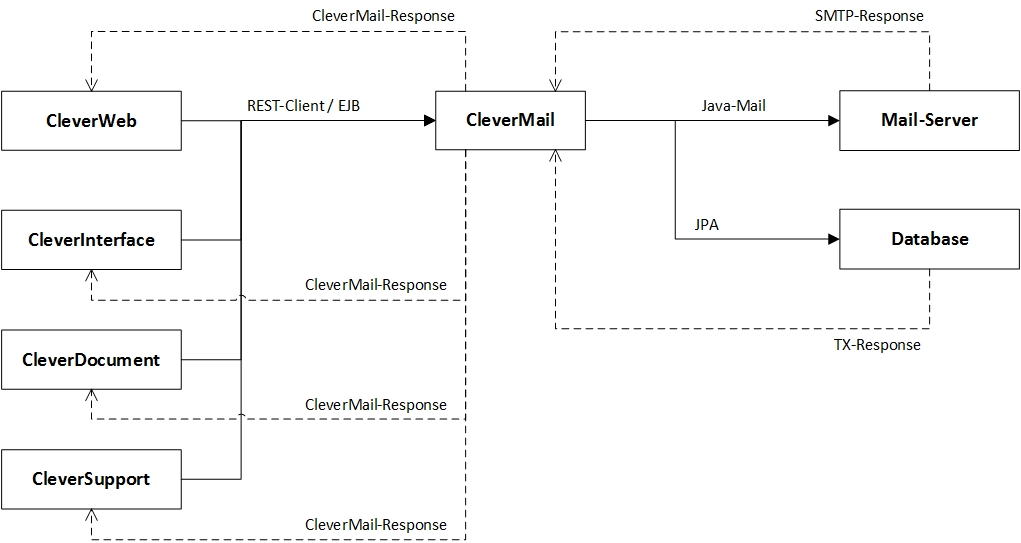
\includegraphics[scale=0.58]{clevermail_systemaufbau.jpg} %{CS0031}
\caption{Systemaufbau und Integration von \emph{CleverMail}}
\label{fig:clevermail-system-und-integration}
\end{figure}
\ \newline
Wie in der Abbildung \ref{fig:clevermail-system-und-integration} illustriert, wird als zentrale Schnittstelle \emph{CleverMail} bzw. dessen implementierte \emph{Client-API} fungieren, wobei diese \emph{Client-API} sich wie folgt ausprägen könnte:
\begin{enumerate}
	\item\emph{REST-Client}, eine REST-Schnittstelle zu einem \emph{REST-Webservice}, über den die zur Verfügung gestellten Funktionalitäten genutzt werden können.
	\item\emph{EJB}, ein EJB (Enterprise Java Bean), welches die zur Verfügung gestellten Funktionalitäten bereitstellt.
\end{enumerate}
\ \newline
\emph{CleverMail} ist für das Persistieren und das Versenden der \emph{E-Mail} verantwortlich und trennt diese Aufgaben vollständig von den Anwendungen. So kann die Wartung an einer Stelle erfolgen und muss nicht über alle Anwendungen hinweg erfolgen. In den Anwendungen würden nur noch Änderungen an den Schnittstellen von \emph{CleverMail} Eingriffe erfordern.
\newline
\newline
Dieser Ansatz würde das Problem der eigens implementierten Datenbankzugriffe beschrieben in Absatz \ref{sec:ccmail-systemaufbau} lösen. Ein Problem könnten hier etwaige technologische Unterschiede darstellen, wie z.B.:
\begin{enumerate}
	\item \emph{REST} nicht verfügbar,
	\item \emph{EJB} nicht verfügbar oder
	\item Falsche Java-Version.
\end{enumerate}
\ \newline
Obwohl diese Probleme auftreten können, kann zumindest gewährleistet werden, dass alle Anwendungen dieselbe Schnittstelle und dasselbe Domänenmodell verwenden, selbst wenn eigene Implementierungen erforderlich sind. Diese Implementierungen würden Softwarekomponenten von \emph{CleverMail} darstellen und dürfen nicht von den Anwendungen selbst bereitgestellt werden.
Diese technologischen Unterschiede könnten wie folgt gelöst werden:
\begin{enumerate}
	\item\emph{REST}, Integration von JAX-RS 2.0. 
	\item\emph{EJB}, Integration eines EJB-Containers, zur Verfügung stellen eines \emph{Wrappers} oder eine eigene Implementierung des spezifizierten Schnittstellen.
\end{enumerate}

\subsection{1. Möglichkeit \emph{(REST-Client)}}
Eine \emph{REST-Client-API}, welche sich mit JAX-RS 2.0 einfach realisieren lässt, würde ein hohes Maß an Abstraktion bieten, nur eine geringe Kopplung aufweisen und wenig Abhängigkeiten in den Anwendungen erfordern, die den \emph{REST-Client} verwenden. Dem steht aber gegenüber, dass \emph{REST-Services} zustandslos sind und sich daher nicht in Datenbank-Transaktionen einbinden lassen. Dies könnte aber erforderlich sein, wenn eine \emph{E-Mail} nur dann angelegt und versendet werden darf, wenn die Transaktion erfolgreich abgeschlossen wurde (z.B. beim Anlegen einer Bestellung). Für einen \emph{REST-Service} startet der Lebenszyklus mit dessen Aufruf und endet mit dem Übermitteln der Antwort oder wenn die Aktion abgeschlossen wurde (asynchron).
\newline
\newline
Für diese Problem gibt es eine Lösung in Form eines Konzeptes mit der Bezeichnung Try-Confirm-Cancel (TCC).
\begin{figure}[h]
\centering
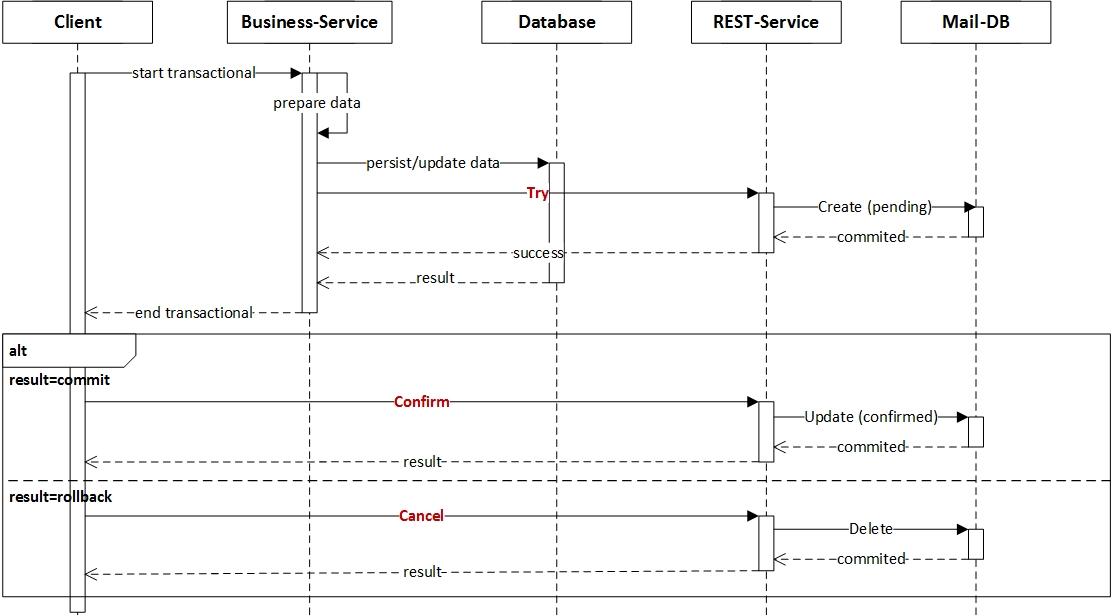
\includegraphics[scale=0.53]{try_confirm_cancel.jpg} %{CS0031}
\caption{Beispiel einer Transaktion mit TCC}
\label{fig:clevermail-rest-tcc}
\end{figure}
\ \newline
Mit dem Konzept \emph{TCC} hält der \emph{REST-Service} die \emph{E-Mail} persistent, markiert die \emph{E-Mail} aber als \emph{unconfirmed}, damit diese \emph{E-Mail} in keiner Verarbeitungslogik miteinbezogen wird. Nach dem erfolgreichen Abschluss der Transaktion auf der \emph{Client}-Seite bestätigt der \emph{Client} den durch den \emph{REST-Service} persistent gehaltenen Zustand, und im Falle eines Fehlers erklärt der \emph{Client} den Zustand für ungültig. Dies erfordert zwei Aufrufe zu REST-Services. Ebenfalls sollte die Transaktion über einen Transaktionskoordinator auf der REST-Seite kontrolliert werden, was wiederum einen Mehraufwand bedeutet. Dieser Transaktionskoordinator wäre dafür verantwortlich, die REST-Services, die Teil einer logischen Transaktionen sind, zu managen. 
\newline
\newline
Mit \emph{TCC} besteht auch die Gefahr das eine \emph{Heuristic-Exception} auftritt. Eine \emph{Heuristic-Exception} tritt auf wenn ein Teilnehmer der Transaktion eine \emph{Heuristic-Decision} (eigenmächtige Entscheidung) trifft und dadurch Dateninkonsistenzen auf der Datenbank entstehen. Dies ist ein Problem, dass vor allem in verteilten System auftreten kann.
\newline
\newline
Diese Probleme bedeuten aber nicht, dass \emph{REST-Services} nicht in Frage kommen. Lediglich für transaktionale Operationen scheinen sie ungeeignet bzw. der Aufwand, der betrieben werden muss, zu hoch. Ein weiteres Problem kann die Erreichbarkeit des \emph{REST-Service} sein. Sollte dieser einmal ausfallen, oder im Falle eines Neuinstallation nicht erreichbar sein, so müsste man eine Rückversicherung haben und die zu erstellenden \emph{E-Mails} anderweitig zwischenspeichern, wie z.B. in Form einer Textdatei, welche die Daten in Form von JSON (Javascript-Objekt-Notation) enthält.
\newline
\newline
Der Artikel \cite{atomikosTcc} beschreibt den Prozess von \emph{TCC} mit mehreren involvierten REST-Services gut und detailliert.

\subsection{2. Möglichkeit \emph{(EJB)}}
Sollte eine Anwendung \emph{CleverMail} via dessen zur Verfügung gestellten \emph{EJBs} verwenden, so würde eine starke Kopplung und starke Abhängigkeiten entstehen, da mehr Ressourcen benötigt werden. Ebenso könnte im Gegensatz zu einem \emph{REST-Client} keine eigene Datenbank genutzt werden, da ein Zweiphasen-\emph{Commit} erfolgen müsste. Natürlich würde die Möglichkeit von mehreren verwendeten Datenbanken bestehen, aber man wäre der Gefahr von \emph{Heursitc-Exceptions} ausgesetzt.
\newpage
\begin{figure}[h]
\centering
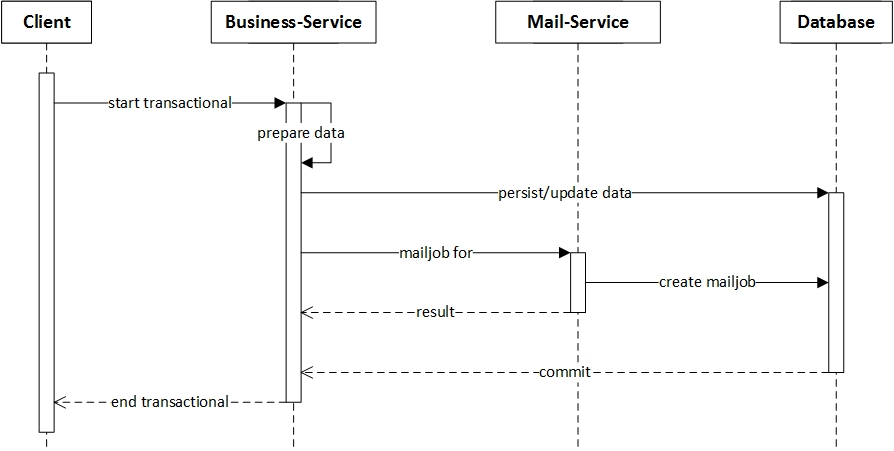
\includegraphics[scale=0.65]{clevermail-ejb-transaktion.jpg} %{CS0031}
\caption{Beispiel einer Datenbanktransaktion mit \emph{EJB}}
\label{fig:clevermail-rest-tcc}
\end{figure}
Wie in Abbildung \ref{fig:clevermail-rest-tcc} illustriert erfolgt das Anlegen einer \emph{E-Mail} in derselben Transaktion und würde daher auch im Falle eines \emph{Rollbacks} entfernt werden. Dies ist sicher die einfachste Art und Weise, um \emph{E-Mails} anzulegen, da hier keine besonderen Mechanismen implementiert werden müssen um die Datenkonsistenz zu gewährleisten. Mit diesem Ansatz wäre die \emph{E-Mail} Teil einer wohldefinierten Transaktion.
\newline
\newline
Wie im Kapitel \ref{cha:clevermail} angemerkt, können technologische Probleme auftreten, wenn z.B. die Laufzeitumgebung einer Anwendung \emph{EJB} und \emph{JTA} nicht zur Verfügung stellt. In so einem Fall müsste man eigene Implementierungen zur Verfügung stellen, die Teil von \emph{CleverMail} sein müssen.
\newline
\newline
Dieser transaktionale Ansatz unterschiedet sich nicht von dem in \emph{CCMail} bereits implementierten, jedoch müssen die von \emph{CleverMail} zur Verfügung gestellten Implementierungen verwendet werden. Diese Implementierungen müssen auch im Backend der \emph{REST-Services} von \emph{CleverMail} verwendet werden, da auch hier die Persistenz der \emph{E-Mails} gewährleistet werden muss.
 
\section{\emph{E-Mail} Prozesse}
\label{sec:clevermail-prozesse}
Dieser Abschnitt behandelt die Prozessspezifikationen von \emph{CleverMail}. Es wird das Augenmerk auf den Mailversand gelegt. Grundlegend wird sich der E-Mail-Versand dadurch unterscheiden, dass mehrere Ebenen involviert sind, bevor eine \emph{E-Mail} bereit zum Versand ist. 
\newline
\newline
Vom grundlegenden Konzept wird sich gegenüber \emph{CCMail} nicht viel ändern. Es soll immer noch E-Mail-Typen geben, die aber jetzt nicht nur intern konfigurierbar sein sollen,  sondern ebenfalls durch die KundInnen selbst konfiguriert und gesteuert werden können. Es sollen folgende Konfigurationsmöglichkeiten zur Verfügung stehen.
\begin{enumerate}
	\item Definition von Zeitplänen.
	\item Definition eigener \emph{E-Mail}-Vorlagen.
	\item Konfiguration der Steuerbarkeit von \emph{E-Mail}-Typen durch LieferantInnen (darf aktivieren/de-aktivieren).
	\item Definition eines Haftungsausschluss. 
	\item Definition von Standard-Datei-Anhängen.
	\item Steuerbarkeit von \emph{E-Mail}-Typen für spezifischen LieferantInnen.
	\item Konzernübergreifende Konfiguration.
	\item Definition eigener E-Mail-Typen.
	\item Konfiguration der Historie der \emph{E-Mail}-Nachrichten.
\end{enumerate}
\ \newline
Zur Zeit stehen diese Features, wenn vorhanden, nur intern zur Verfügung. Die Kunden haben lediglich die Möglichkeit einzelne E-Mail-Typen zu aktivieren oder zu de-aktivieren. Diese E-Mail-Typen können aber mehrere E-Mail-Nachrichten beinhalten. Das Grundlegende Ziel ist dass die Kunden mehr Kontrolle und Konfigurationsmöglichkeiten über die zur Verfügung gestellten E-Mail-Typen erhalten. Es wird hier aber auch solche E-Mail-Typen geben, bei denen diese Konfigurationsmöglichkeiten eingeschränkt werden. Nichts desto trotz soll der Kunde in der Lage sein, den E-Mail-Verkehr seiner E-Mail-Nachrichten besser zu steuern.

\newpage
\subsection{E-Mail-Versand}
\begin{figure}[h]
\centering
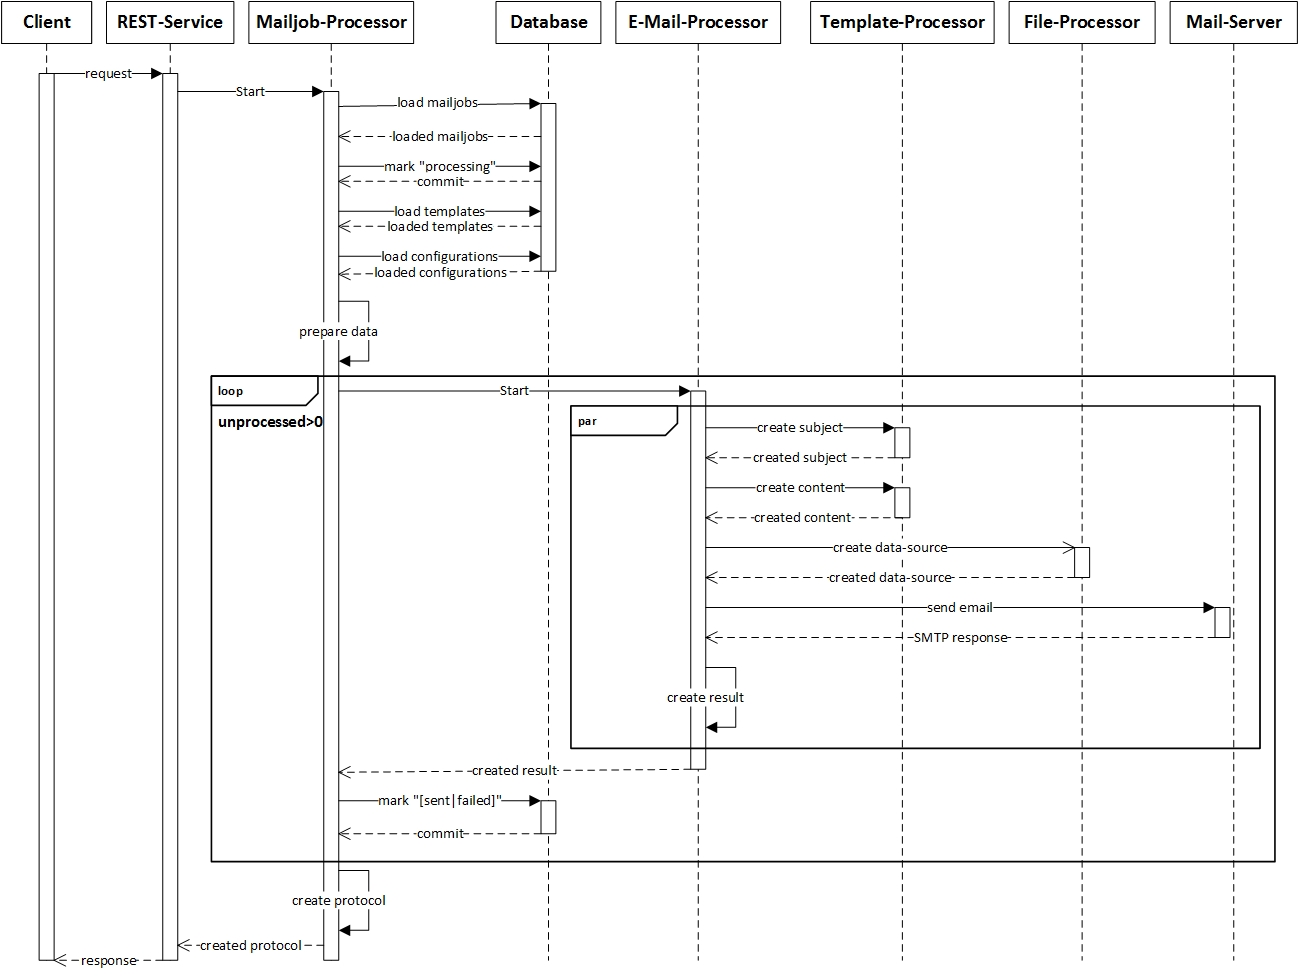
\includegraphics[angle=90, scale=0.6]{clevermail-email-versand.jpg} %{CS0031}
\caption{Prozess des E-Mail-Versands}
\label{fig:clevermail-email-versand}
\end{figure}
\ \newpage
Die Abbildung \ref{fig:clevermail-email-versand} soll den Prozess des E-Mail-Versands veranschaulichen und illustriert die Softwarekomponenten, die involviert sind um eine E-Mail-Nachricht zu erstellen. In diesem Beispiel wird der Prozess über einen REST-Service gestartet, der in diesem Fall den Prozess synchron abarbeitet und anschließend eine Response in Form eines erstellten Reports zurückliefert. Der REST-Service ist hierbei als optional anzusehen, da dieser Prozess auch anderweitig ausgelöst werden könnte. Nachdem sich dieser Prozess nicht in einer Transaktion eines Client befinden muss würde sich hier eine REST-Schnittstelle anbieten.
\newline
\newline
Folgende sei der Prozess in grobe Schritte unterteilt angeführt und beschrieben.

\subsubsection{Daten Aufbereitung}
Nachdem der Prozess gestartet wurde sollen die zu verarbeitenden E-Mail-Nachrichten aus der Datenbank ausgelesen und als \emph{Processing} markiert werden. Im Punkt \ref{sec:ccmail-email-versand} wurde angemerkt, dass das Problem bestand, dass die in Verarbeitung stehenden \emph{MailJob} Entitäten nicht als solche markiert wurden und daher eine parallele Verarbeitung durch mehrere Prozesse nicht möglich war. Dieses Problem besteht in diesem Fall nun nicht mehr. Nachdem die \emph{MailJob} geladen wurden sollen die zugrunde liegenden E-Mail-Vorlagen geladen werden. Hierbei würde sich ein Cache-Mechanismus auszahlen, da die E-Mail-Vorlagen Versionen definieren sollen und sich innerhalb einer Version nicht mehr ändern dürfen. Anschließend sollen die kundenspezifischen Konfigurationen geladen werden. Aus diesen Daten sollen Modelle erstellt werden, die in weitere Folge dazu verwendet werden sollen die E-Mail-Nachrichten zu erstellen.

\subsubsection{Erstellen der E-Mail-Nachrichten}
Aus den Modellen sollen die E-Mail-Nachrichten erstellt werden. Hierbei wird dieser Prozess in drei Schritte unterteilt.
\begin{enumerate}
	\item\emph{Erstellen des Betreff}
	\newline
	Der Betreff wird aus einer E-Mail-Vorlage erstellt und mit Daten befüllt wenn in der Voralge Parameter definiert wurden
	\item\emph{Erstellen der Nachricht}
	\newline
	Die Nachricht wird aus einer E-Mail-Vorlage erstellt und mit Daten befüllt wenn in der Voralge Parameter definiert wurden
	\item\emph{Erstellen der DataSoruces}
	\newline
	Sollten Datei Anhänge definiert worden sein, so werden diese in Form von einer oder mehrerer DataSoruce Instanzen in die E-Mail-Nachricht angefügt.
\end{enumerate}
\ \newline
Die Verarbeitung der E-Mail-Vorlagen soll in einer Komponente mit dem Name \emph{Template-Processor} erfolgen. Nachdem die Werte der verwendeten Vorlagenparameter beim Erstellen eines \emph{MailJob} in der Datenbank gespeichert wurden können diese hier angewandt werden.
\newline
\newline
Die Verarbeitung der Datei Anhänge soll in einer Komponente mit dem Namen \emph{File-Processor} erfolgen, die die verlinkten Datei Anhänge in Form von \emph{DataSource} Instanzen der E-Mail-Nachricht zur Verfügung stellt. Beim Versand würde die E-Mail-Nachricht den Datei Anhang über diese \emph{DataSource} Instanz laden. Hierbei sollen die Dateien in Form von Links aus dem Dokumentenmanagementsystem \emph{CleverDocument} geladen werden. Es sollen keine Dateien in Form von Base64-Zeichenketten in der Datenbank gespeichert werden, um die Datenbank nicht mit unnötigen Daten zu belasten. Es könnten hierbei verschiedene \emph{DataSource} Implementierungen zur Verfügung gestellt werden, die die Dateien aus verschiedenen Quellen über die verschiedensten Protokolle laden können (z.B.: REST, SOAP, HTTP, usw.).

\subsubsection{E-Mail versenden}
Der E-Mail-Versand sowie das Erstellen der E-Mail-Nachricht sollte hierbei asynchron erfolgen, da eine sequenzielle Verarbeitung die Performance negativ beeinflussen würde. Nach dem erfolgreichen oder fehlgeschlagenen Versand einer E-Mail-Nachricht soll dieser Status in Form eines Resultates zurückgeliefert werden. Hierbei ist vor allem die SMTP-Response wichtig, die auf jeden Fall gespeichert werden soll, damit der Kunde nachvollziehen kann, wie der E-Mail-Versand seiner E-Mail abgearbeitet wurde und warum die E-Mail nicht zugestellt werden konnte. Ein fehlgeschlagener Versand könnte folgende Ursachen haben:
\begin{enumerate}
	\item Datei kann nicht geladen werden (nicht vorhanden, Timeout,...)
	\item Mail-Server des Empfängers nicht erreichbar
	\item E-Mail-Server nimmt Nachricht nicht an
	\item uvm.
\end{enumerate}
\ \newline
Es kann unzählige Ursachen haben warum eine E-Mail-Nachricht nicht zugestellt werden kann. Die trifft vor allem auf den E-Mail-Servers des Empfängers zu, auf dessen Konfiguration kein Einfluss genommen werden kann.

\newpage
\subsection{E-Mail-Vorlagen(parameter)}
Ein weiterer wichtiger Aspekt stellen die Vorlagen und dessen zur Verfügung gestellten Parameter und deren Verwaltung dar. Die Bereitstellung von Vorlagenparametern soll den AnwenderInnen die Möglichkeit bieten auf kontextabhängige Daten in einer E-Mail-Vorlage zugreifen zu können. Dadurch soll die Flexibilität erhöht werden und die AnwenderInnen sollen mehr Freiheiten beim Erstellen einer E-Mail-Vorlage bekommen. Diese Parameter müssen hierbei von den EntwicklerInnen innerhalb eines Kontextes zur Verfügung gestellt werden, wobei hier auch ein Entwicklungsaufwand besteht. Diese Parameter müssen beim Verarbeiten einer E-Mail-Vorlage aus dem aktuellen Kontext ausgelesen werden. Dabei können die Daten aus verschiedenen Objekten oder sogar Objektgraphen kommen. Dies bedeutet dass diese Parameter über eine spezielle Implementierung ausgelesen werden müssen, die auch zukünftig gewartet werden muss. Ebenso werden diese Parameter in verschiedenen Softwarekomponenten verwendet, die sich in verschiedenen Laufzeitumgebungen befinden können. Daher wird es erforderlich sein diese Parameter in einem spezifizierten Model oder über definierte Zuordnungen von einem Model in ein anderes Model zu überführen.
\begin{figure}[h]
\centering
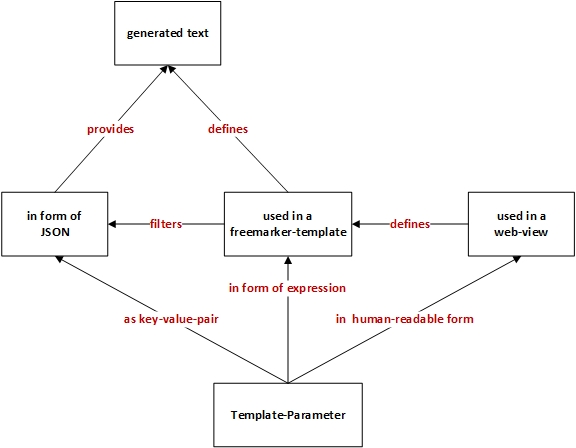
\includegraphics[scale=0.6]{clevermail_template_parameter.jpg}
\caption{Verwendung Vorlagenparameter}
\label{fig:clevermail-template-parameter}
\end{figure}
\ \newline
Wie in der Abbildung \ref{fig:clevermail-template-parameter} illustriert werden die Vorlagenparameter in mehreren Kontexten verwendet. Dadurch stellt sich die Frage wie diese Parameter adressiert werden. Man könnte eine Zuordnung in jedem Verwendungskontext erstellen, also jeder Kontext bekommt sein eigenes Model. Dadurch würde man sich zwar lose and die Vorlagenparameter koppeln jedoch erhält man auch eine Model Klasse je Kontext, die gewartet werden muss. 

\subsubsection{Webseite}
\label{sec:template-parameter-web-view}
Da diese Parameter in E-Mail-Vorlagen verwendet werden wird es auch eine Webseite geben, über die die AnwenderInnen diese Parameter in Ihren E-Mail-Vorlagen verwenden können. Diese müssen natürlich für die AnwenderInnen einen Name bekommen, der natürlich auch in mehreren Sprachen zur Verfügung stehen muss. Dadurch werden diese Parameter auf einen Schlüssel zugeordnet werden müssen, der wiederum auf einen lokalisierten Spracheintrag zugeordnet ist. Die Zuweisung auf diesen Schlüssel ist erforderlich aber benötigt man hier auch nochmals eine Zuordnung auf den Vorlagenparameter?

\subsubsection{Freemarker}
\label{sec:template-parameter-freemarker}
Ein weiterer Aspekt ist auch die direkte Verwendung der Parameter in der Vorlage selbst. Als Implementierung einer \emph{Template-Enging} soll für die Erstellung der Nachrichten aus den Vorlagen \emph{Freemarker}\footnote{\label{fn:freemarker}Frei verfügbare Template-Engine in Java für die Erstellung von dynamischen Textdateien} verwendet werden. Dieses Framework ist ein sehr beliebtes und gut gewartetes Framwork, welches alle benötigten Kontrollstrukturen sowie \emph{Freemarker-Expressions} zur Verfügung stellt. Diese \emph{Freemarker-Expressions} ähneln sehr den Java-EL-Expressions\footnote{Java-Expression-Language ist eine Java Spezifikation für Expressions}. 
Die Vorlagenparameter werden in den \emph{Freemarker-Expressions} verwendet, die es ermögliche eine flache Adressierung sowie auch eine Adressierung über Objektgraphen zu definieren. Dadurch stellt sich auch hier die Frage ob diese Expressions wieder über eine Zuordnung zu den Parametern erstellt werden sollen oder ob die Parameter selbst verwendet werden sollen?

\subsubsection{JSON}
\label{sec:template-parameter-json}
Wenn eine E-Mail in Form eines \emph{MailJob} erstellt wird müssen zum jeweiligen Erstellungszeitpunkt alle Parameterwerte ausgelesen und mit dem \emph{MailJob} persistent gehalten werden. Nachdem die Anzahl der Parameter dynamisch ist und diese Daten lediglich in der Vorlagenverarbeitung verwendet werden ist es hier nicht erforderlich eine eigene Datenstruktur auf der Datenbank zu definieren. Dadurch würde sich hier \emph{JSON} anbieten um diese Daten in die Datenbank zu serialisieren. Nachdem \emph{JSON} eine Objektbeschreibung darstellt und auch über ein \emph{JSON-Schema} spezifiziert werden kann, sollte man überlegen ob man nicht das \emph{JSON} als Spezifikation für die Vorlagenparameter heranzieht. Diese Spezifikation kann in allen involvierten Komponenten verwendet werden. 

\newpage
\section{Datenbank}
Neben der Persistenz der E-Mail-Nachrichten soll ebenfalls die Möglichkeit bestehen, den E-Mail-Versand zu konfigurieren. Dies soll einerseits Firmen intern möglich sein und andererseits auch für die AnwenderInnen. Hierbei sollen folgende Möglichkeiten zur Verfügung stehen:
\begin{enumerate}
	\item Zeitsteuerung des Versandes
	\item Berechtigungen für Modifikationen der E-Mail-Nachrichten
	\item Eigene E-Mail-Typen
	\item Eigene E-Mail-Vorlagen
	\item Zusatzdokumente 
	\item Speicherverwaltung der E-Mail
\end{enumerate}
\ \newline
Um diese Konfigurationen zu verwalten wird ein Speichermedium benötigt, welches ebenfalls in der Lage ist die Relationen abzubilden. Da bietet sich verständlicherweise eine Datenbank an. Dies wurde bereits in der alten Anwendung \emph{CCMail} so angewandt und soll auch hier fortgeführt werden. Hierbei soll aber das bestehende Datenbankschema nicht berücksichtigt werden und ein neues konzipiert werden. Im Gegensatz zu dem bestehenden Datenbankschema beschrieben im Punkt \ref{sec:ccmail-datanbank} soll hierbei keineswegs auf die referenzielle Integrität zwischen den involvierten Tabellen verzichtet werden. Dies stellt die größte Fehlentscheidung beim Design des Datenbankschemas dar. Des weiteren soll so gut wie möglich auf die Unabhängigkeit des Datenbankschemata geachtet werden. Hierbei ist gemeint dass die Tabellen des Schemata für \emph{CleverMail} nicht in bestehende Tabellen der Anwendung \emph{Clevercure} referenzieren sollen. Damit soll sichergestellt werden, dass dieses Datenbankschema auch als Standalone verwendet werden kann. Sollten Referenzen auf Tabellen wie Benutzer (USER), Kunde (COMPANY) des \emph{Clevercure} Datenbankschema eingeführt werden, so kann \emph{CleverMail} nicht außerhalb des Kontextes von \emph{Clevercure} existieren und würde immer nur für diese Anwendung zur Verfügung stehen. Das Modul \emph{CleverMail} sollte aber auch als Standalone-Anwendung funktionsfähig sein, auch wenn es für die Anwendung \emph{Clevercure} entwickelt werden soll. Diese begründet sich durch die Anwendungsfälle selbst, die nicht auf eine bestimmte Repräsentation von Inhabern von persistenten E-Mail-Nachrichten, E-Mail-Typen oder Konfigurationen angewiesen sind. Mann sollte sich hier die Möglichkeiten für eine zukünftige Anwendung in anderen Anwendungen offen halten anstatt sich den Aufwand einer umfangreichen Refaktorisierung beim Eintreffen eines solchen Falles auszusetzen. 
\newline
\newline
Auch wenn dieser Ansatz verfolgt werden soll ist es natürlich auch möglich diese Referenzen herzustellen solange der Datenzugriff gekapselt nur einer Stelle oder voll definierten Stellen stattfindet. Somit ist gewährleistet, dass eine Refaktorisierung keine unerwünschten Nebeneffekte hat und man nicht vergisst Änderungen an Stellen nachzuziehen, die vergessen wurden. Dies kann leicht passieren wenn solche Implementierungsteile beim Refaktorisieren nicht bekannt sind. Scott W.Ambler und Parmond J.Sadalage beschreiben dies in Ihrem Buch 
\emph{Refactoring Databases} \cite[66]{refactoreDatabase} wie folgt.
\begin{quote}
\emph{You could implement the SQL logic in a consistent manner, such as having save(), delete(), retrieve(), and find() operations for each business class. Or you could implement data access objects(DAOs), classes that impleemnt the data access logic separately from business classes.}
\end{quote}
Natürlich ist der Ansatz mit \emph{DAOs} vorzuziehen, da hier der Datenzugriff gekapselt an einer Stelle implementiert wird und nicht zerstreut über n-Business-Klassen implementiert wird.
\newpage
\subsection{Datenbankschemata CleverMail}
\begin{figure}[h]
\centering
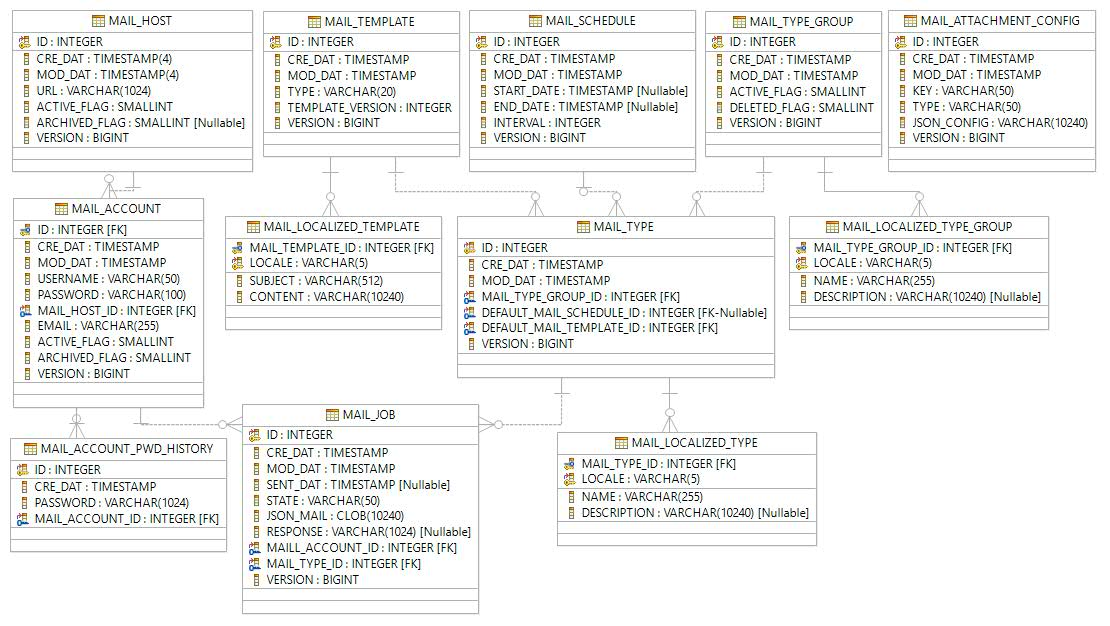
\includegraphics[angle=90, scale=0.4]{clevermail_db_schema.jpg}
\caption{Datenbankschema CleverMail}
\label{fig:clevermail-db-schema}
\end{figure}
Das angeführte Datenbankschema \ref{fig:clevermail-db-schema} stellt eine mögliche Implementierung des Datenbankschemata dar. Dieses Datenbankschema enthält keine Referenzen auf das Datenbankschema von \emph{Clevercure}. Die Integration in das Datenbankschema von \emph{Clevercure} bzw. die Integration des Datenbankschemata von \emph{Clevercure} in das Datenbankschemata von \emph{CleverMail}, wie im diesen Beispiel angedacht, könnte über N-M-Tabellen abgebildet werden. Mit dieser Art der Tabellenrelation kann auch eine 1-N Relation abgebildet werden, wobei noch zusätzlich ein Unique-Constraint auf den Forgein-Key der referenzierten Tabelle hinzugeüfgt werden muss. Mann erhält mit diesem Ansatz zwar noch zusätzliche Relationstabellen, die ebenfalls einen zusätzlichen Join erfordern, jedoch ist so sichergestellt, dass das Datenbankschemata von \emph{CleverMail} unabhängig bleibt.
\newline
\newline
Es ist auch anzumerken, dass das Datenbankschemata \ref{fig:clevermail-db-schema} von \emph{CleverMail} sehr dem Datenbankschemata \ref{fig:ccmail-db-schema} ähnelt. Wobei natürlich neue Tabellen hinzugefügt wurden um die neuen Features wie die Steuerbarkeit des E-Mail-Versandes zu unterstützen. Nicht desto Trotz finden sind viele Eigenschaften von \emph{CCMail} wieder mit einen etwas anderen Ansatz sowie natürlich auch der Umsetzung.